
\section{Position-Angle Experiment}

The position-angle experiment was originally performed by Cleveland and McGill to measure whether humans can better perceive quantities encoded as positions or as angles~\cite{cleveland_mcgill}. The actual experiment then compares pie charts versus bar charts since these map down to elementary position and angle judgement. We create rasterized images mimicking Cleveland and McGill's proposed encoding and investigate computational perception of our four classifiers.

%\begin{figure}[t]
%	  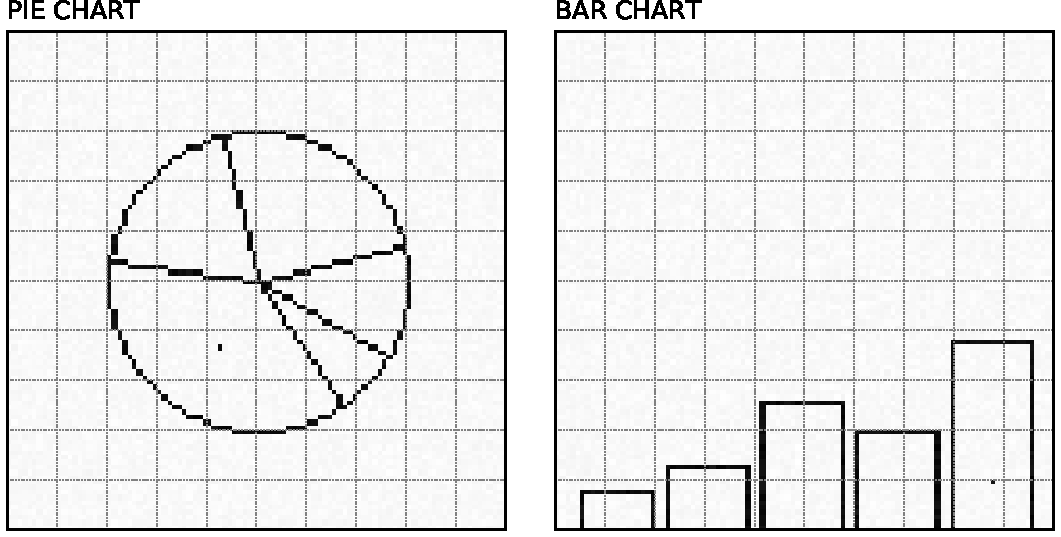
\includegraphics[width=\linewidth]{figure3_overview}
%  \caption{\textbf{Position-Angle Experiment.} We create rasterized visualizations of pie charts and bar charts to follow Cleveland and McGill's position-angle experiment. The experimental task involves the judgement of different encoded values in comparison to the largest encoded values. The pie chart (left) and the bar chart (right) visualize the same data point. In their paper, Cleveland and McGill report less errors using bar charts.}
%	\label{fig:position_angle_experiment}
%\end{figure}
\begin{table}[h]
\centering
\caption{\textbf{Position-Angle Experiment.} We create rasterized visualizations of pie charts and bar charts to follow Cleveland and McGill's position-angle experiment. The experimental task involves the judgement of different encoded values in comparison to the largest encoded values. The pie chart and the bar chart visualize the same data point. In their paper, Cleveland and McGill report less errors using bar charts.}
\resizebox{\linewidth}{!}{
\begin{tabular}{lllr}
	\toprule
	\multicolumn{2}{l}{~} & ~ & Permutations\\

	\midrule
	\raisebox{-.85\height}{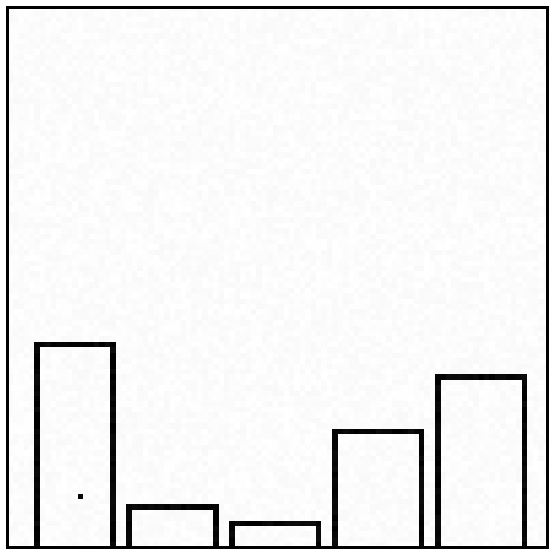
\includegraphics[width=.5in]{figure3_Bar_Chart.pdf}} & \makecell[tl]{Type 1: \emph{Bar Chart}\\~~~Perceptual Task: \emph{Position}\\~ \\~ \\} &~& \makecell[tr]{~\\ $244,827$}\\


	\midrule
	\raisebox{-.85\height}{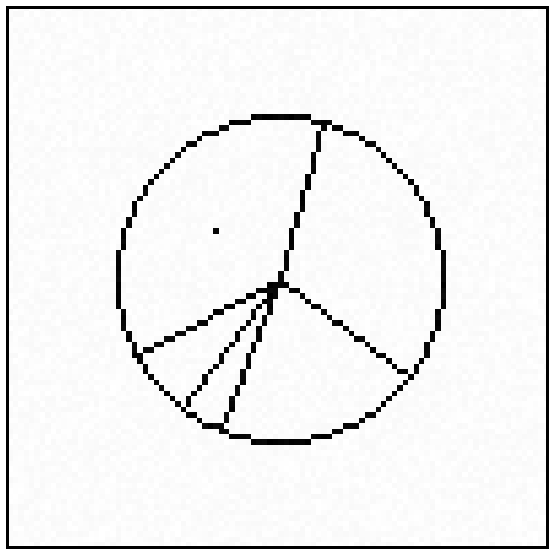
\includegraphics[width=.5in]{figure3_Pie_Chart.pdf}} & \makecell[tl]{Type 2: \emph{Pie Chart}\\~~~Perceptual Task: \emph{Angle}\\~ \\~ \\} &~& \makecell[tr]{~\\ $244,827$}\\


	\bottomrule
\end{tabular}
}
\label{tab:pos_angle_parameters}
\end{table}

\subsection{Hypotheses}

We proposed four hypotheses entering the elementary perceptual task experiment:

\begin{itemize}
	\item \textbf{H2.1} \textbf{Computed perceptual performance is better using bar charts than pie charts.} Cleveland and McGill report that position judgements are almost twice as accurate as angle judgements. This renders bar charts superior to pie charts and should also be the case for convolutional neural networks.
	\item \textbf{H2.2} \textbf{Classifiers can learn position faster than angles.} We assume that understanding bar charts is easier than understanding pie charts. We suspect that our classifiers learn encodings of positions faster than of angles resulting in more efficient training and faster convergence.
\end{itemize}

\subsection{Results}


Bar charts are more accurate (Fig.~\ref{fig:figure3_mlae}) and networks converge faster (Fig.~\ref{fig:figure3_val_loss}). This is great.

\begin{figure}[t]
	  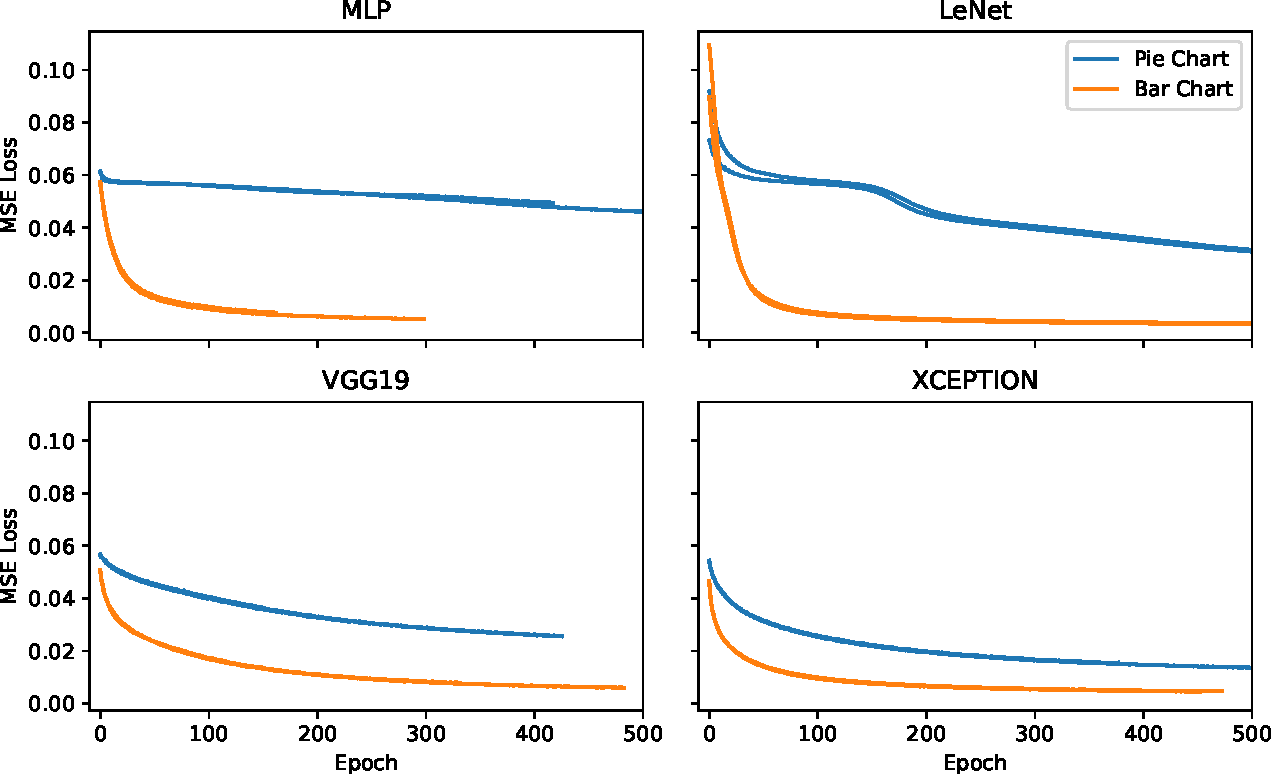
\includegraphics[width=\linewidth]{figure3_val_loss.pdf}
  \caption{\textbf{Classifier Efficiency of the Position-Angle experiment.} Mean Square Error (MSE) loss for the \emph{position-angle experiment} as described by Cleveland and McGill~\cite{cleveland_mcgill} which compares the visualization of pie charts and bar charts. We report the MSE measure for both encodings of four different classifier on previously unseen validation data.}
	\label{fig:figure3_val_loss}
\end{figure}

\begin{figure}[t]
	  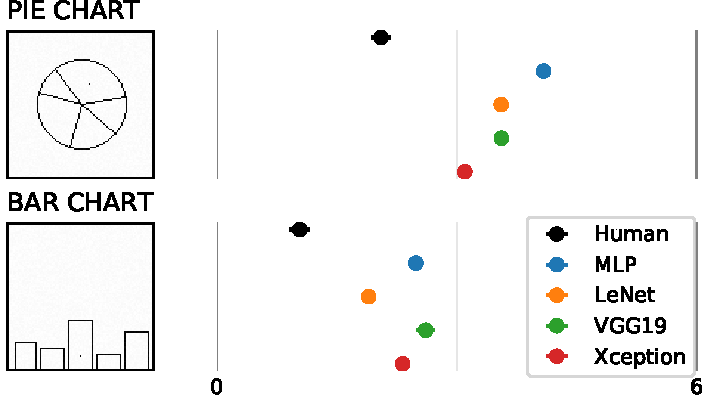
\includegraphics[width=.8\linewidth]{figure3_mlae_better.pdf}
  \caption{\textbf{Computational results of the Position-Angle experiment.} Log absolute error means and 95\% confidence intervals for the \emph{position-angle experiment} as described by Cleveland and McGill~\cite{cleveland_mcgill}. We test the performance of a Multi-layer Perceptron (MLP), the LeNet Convolutional Neural Network, as well as feature generation using the VGG19 and Xception networks trained on ImageNet.}
	\label{fig:figure3_mlae}
\end{figure}
